\documentclass[a4paper,parskip,11pt, DIV12]{scrreprt}

\usepackage[english]{babel} % FÌr Deutsch [english] zu [ngerman] Àndern. 
\usepackage[utf8]{inputenc}
\usepackage[T1]{fontenc}
\usepackage{blindtext}
\usepackage{graphicx}
\usepackage{subfigure}
%\renewcommand{\familydefault}{\sfdefault}
\usepackage{fancyhdr}
\usepackage{amsmath}
\usepackage{mdwlist} %Benötigt fÌr AbstÀnde in AufzÀhlungen zu löschen
\usepackage{here}
\usepackage{calc}
\usepackage{hhline}
\usepackage{marginnote}
\usepackage{chngcntr}
\usepackage{helvet}
\usepackage{tabularx}
\usepackage{titlesec} % TextÃŒberschriften anpassen
\setkomafont{sectioning}{\rmfamily}{\bfseries}

% \titleformat{Überschriftenklasse}[Absatzformatierung]{Textformatierung} {Nummerierung}{Abstand zwischen Nummerierung und Überschriftentext}{Code vor der Überschrift}[Code nach der Überschrift]

% \titlespacing{Überschriftenklasse}{Linker Einzug}{Platz oberhalb}{Platz unterhalb}[rechter Einzug]

\titleformat{\chapter}{\LARGE\bfseries}{\thechapter\quad}{0pt}{}
\titleformat{\section}{\Large\bfseries}{\thesection\quad}{0pt}{}
\titleformat{\subsection}{\large\bfseries}{\thesubsection\quad}{0pt}{}
\titleformat{\subsubsection}{\normalsize\bfseries}{\thesubsubsection\quad}{0pt}{}

\titlespacing{\chapter}{0pt}{-2em}{6pt}
\titlespacing{\section}{0pt}{6pt}{-0.2em}
\titlespacing{\subsection}{0pt}{5pt}{-0.4em}
\titlespacing{\subsubsection}{0pt}{-0.3em}{-1em}

%\usepackage[singlespacing]{setspace}
%\usepackage[onehalfspacing]{setspace}

\usepackage[
			%includemp,				%marginalien in Textkörper einbeziehen
			%includeall,
			%showframe,				%zeigt rahmen zum debuggen		
			marginparwidth=25mm, 	%breite der marginalien
			marginparsep=5mm,		%abstand marginalien - text
			reversemarginpar,		%marginalien links statt rechts
			%left=50mm,				%abstand von Seitenraendern
%			top=25mm,				%
%			bottom=50mm,
			]{geometry}		

%Bibliographie- Einstellungen
\usepackage[babel,german=quotes]{csquotes}
\usepackage[
   backend=bibtex8, 
   natbib=true,
    style=numeric,
    sorting=none
]{biblatex}
\bibliography{Quelle}
%Fertig Bibliographie- Einstellungen

\usepackage{hyperref}

\newcommand{\footnoteremember}[2]{
  \footnote{#2}
  \newcounter{#1}
  \setcounter{#1}{\value{footnote}}
}
\newcommand{\footnoterecall}[1]{%
  \footnotemark[\value{#1}]
}
	
\begin{document}
	
	\begin{titlepage}
		\begin{figure}[H]
			\hfill
			\subfigure{
\includegraphics[scale=0.04]{uzh}}
		\end{figure}
		\vspace{1 cm}
		\textbf{\begin{huge}KT I Lab Course
		\end{huge}}\\
		\noindent\rule{\textwidth}{1.1 pt} \\
		
		\begin{Large}\textbf{Angular Correlation}
		\end{Large}\\ 
		\normalsize 
		\par
		\begingroup
		\leftskip 0 cm
		\rightskip\leftskip
		\textbf{Assistant:}\\ Alexander Kish \\ \\
		\textbf{Students:}\\ Fabian Stäger, Manuel Sommerhalder \\ \\
		\textbf{Date of experiment:}\\ 24.01.2018 \\ \\
		\par
		\endgroup
		\clearpage
		
		
		
	\end{titlepage}
	
%Start Layout
	\pagestyle{fancy}
	\fancyhead{} 
	\fancyhead[R]{\small \leftmark}
	\fancyhead[C]{\textbf{Angular Correlation} } 
	\fancyhead[L]{
\includegraphics[height=2\baselineskip]{uzh}}
	
	\fancyfoot{}
	\fancyfoot[R]{\small \thepage}
	\fancyfoot[L]{}
	\fancyfoot[C]{}
	\renewcommand{\footrulewidth}{0.4pt} 
	
	\addtolength{\headheight}{2\baselineskip}
	\addtolength{\headheight}{0.6pt}
	
	
	\renewcommand{\headrulewidth}{0.6pt}
	\renewcommand{\footrulewidth}{0.4pt}
	\fancypagestyle{plain}{				% plain redefinieren, damit wirklich alle seiten im gleichen stil sind (ausser titlepage)
		\pagestyle{fancy}}
	
	\renewcommand{\chaptermark}[1]{ \markboth{#1}{} } %Das aktuelle Kapitel soll nicht Gross geschriben und Nummeriertwerden
	
	\counterwithout{figure}{chapter}
	\counterwithout{table}{chapter}
	%Ende Layout
	
	\tableofcontents
	
\chapter{Introduction}

		The goal of this experiment is to measure the angular correlation function of $\gamma$-rays in a $^{60}$Co decay and compare it to theoretical predictions.

\section{The $^{60}$Co Decay}

		$^{60}$Co is a synthetic isotope of cobalt with a half-life of 5.1 years. Through $\beta ^-$ decay it disintegrates into an excited $^{60}$Ni atom with an energy of 2505 keV and $l$ = 4 with positive parity. This nickel isotope thus emits two successive gamma rays with energies of 1172 keV and 1332 keV in order to reach its stable state of 0$^{+}$. Since the intermediate state (2$^+$) has a lifetime of around 1 ps, the two $\gamma$-rays can due to the finite experimental time resolution be treated as coincident. A schematic diagram of the $^{60}$Co decay is provided in figure \ref{fig:CoDecay}.	
\begin{figure}[H]
\centering
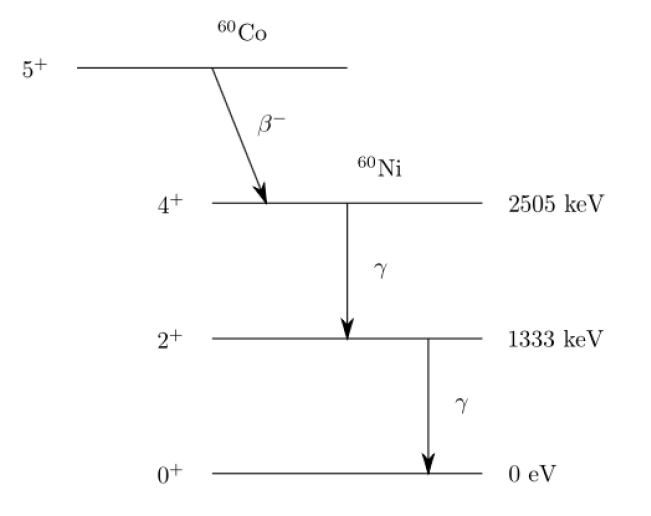
\includegraphics[scale=0.65]{60CoDecay.png}
\caption[60CoDecay]{Schematic illustration of the $^{60}$Co Decay. [\ref{source:manual}]}
\label{fig:CoDecay}
\end{figure}
		
\section{Angular Correlation}

		The two successive $\gamma$-rays are predicted to be emitted anisotropically relative to each other according to the general angular correlation function [\ref{source:manual}]:
		\begin{equation}
		W(\theta) = 1 + \sum^l_1 a_i \cos ^{2i} \theta
		\end{equation}	
		This function describes the probability for the latter gamma ray to be emitted at an angle $\theta$ from the first one. 2$l$ is the order of the lowest multipole in the cascade. In case of the $^{60}$Co decay, both gamma rays are emitted during a transision of $\Delta l$ = 2 and positive parity, so the dominant contribution is the electric quadrupole and the correlation function reduces to:	
		\begin{equation}
		W(\theta) = 1 + a_1 \cos ^{2} \theta +  a_2 \cos ^{4} \theta
		\end{equation}		
		The coefficients $a_1$ and $a_2$ have been theoretically predicted by Dr. Hamilton for all combinations of angular momenta involved by consideration of state transitions using the Clebsch-Gordan-coefficients. These are summarized in figure \ref{fig:coefficients}		
		\begin{figure}[H]
\centering
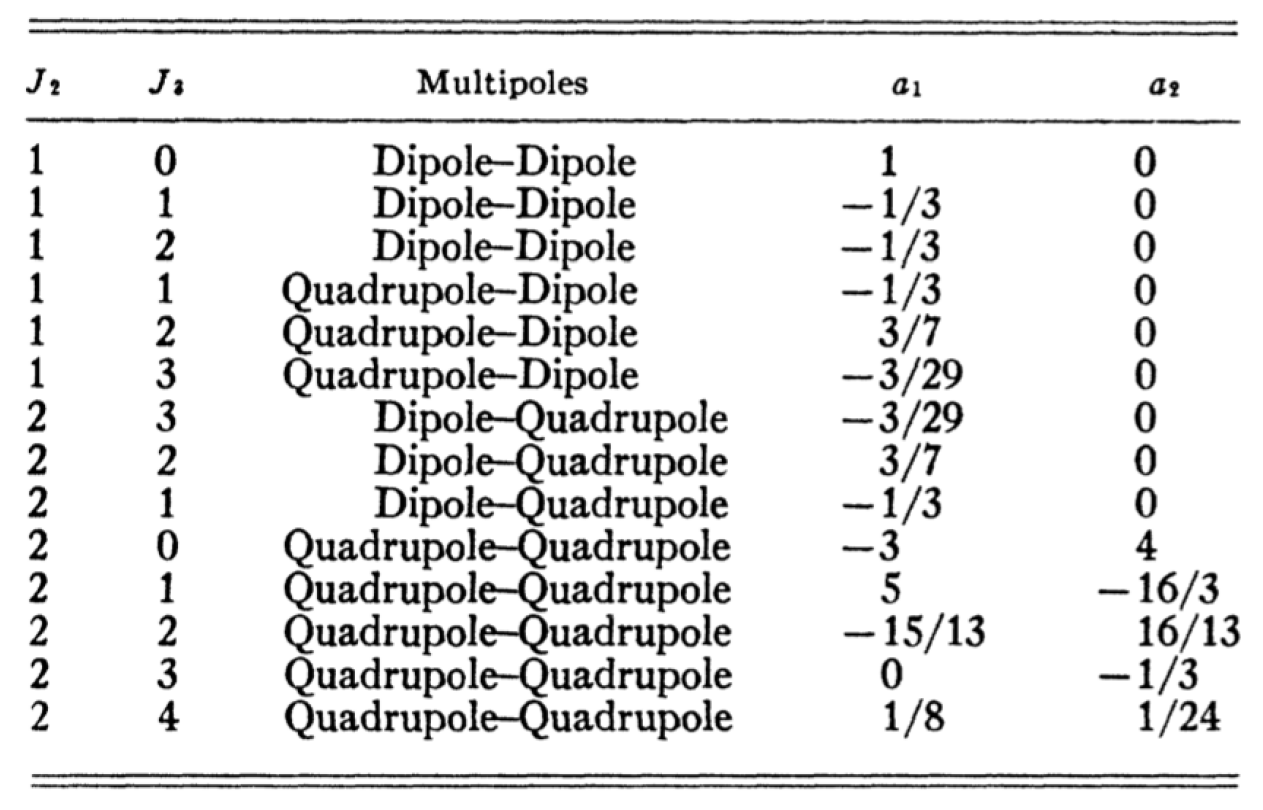
\includegraphics[scale=0.4]{Coefficients.png}
\caption[Coefficients]{Coefficients $a_1$ and $a_2$ for different combinations of $J_1$ and $J_2$ for an atom deexciting into the ground state $J_1$ = 0 [\ref{source:manual}]}
\label{fig:coefficients}
		\end{figure}		
		Since the angular monenta of $J_3$ = 4, $J_2$ = 2, $J_1$ = 0 are assumed for the $^{60}$Co decay, the expected correlation function has the following explicit form:		
		\begin{equation} \label{eq:AngularCorrelation}
		W(\theta) = 1 + \frac{1}{8} \cos ^{2} \theta +  \frac{1}{24} \cos ^{4} \theta
		\end{equation} 
		
\section{Experimental Concept}

		The experimental setup, more throroughly described in section \ref{sec:setup}, consists of two scintillation counters that detect the coincident $\gamma$-rays from different and adjustable relative angles. The rate of detected events is then plotted and compared to the theoretical description from formula \ref{eq:AngularCorrelation}.
		
\chapter{Measurement Principle}	

\section{Experimental Set-Up}

\section{Electronic Modules}

\chapter{Energy Spectrum} \label{sec:EnergySpectrum}

		Figure \ref{fig:EnergySpectra} shows the energy spectra measured at the two detectors correspondingly where the horizontal axis has been rescaled compared to he original measurement in figure \ref{fig:EnergySpectraUnscaled} in the appendix. In the original measurement, the number of events was a function of channels whose absolute values do not have any physical meaning. The two sharp peaks in the right half of the plot could be easily identified as the typical $\gamma$-decay absorption lines. Their corresponding energy values of $E_{\gamma,1}$ = 1172 keV and $E_{\gamma}$ = 1332 keV are well known in the literature and were used for the energy calibration that made the rescaling to energy units possible.	
		\begin{figure}[H]
\centering
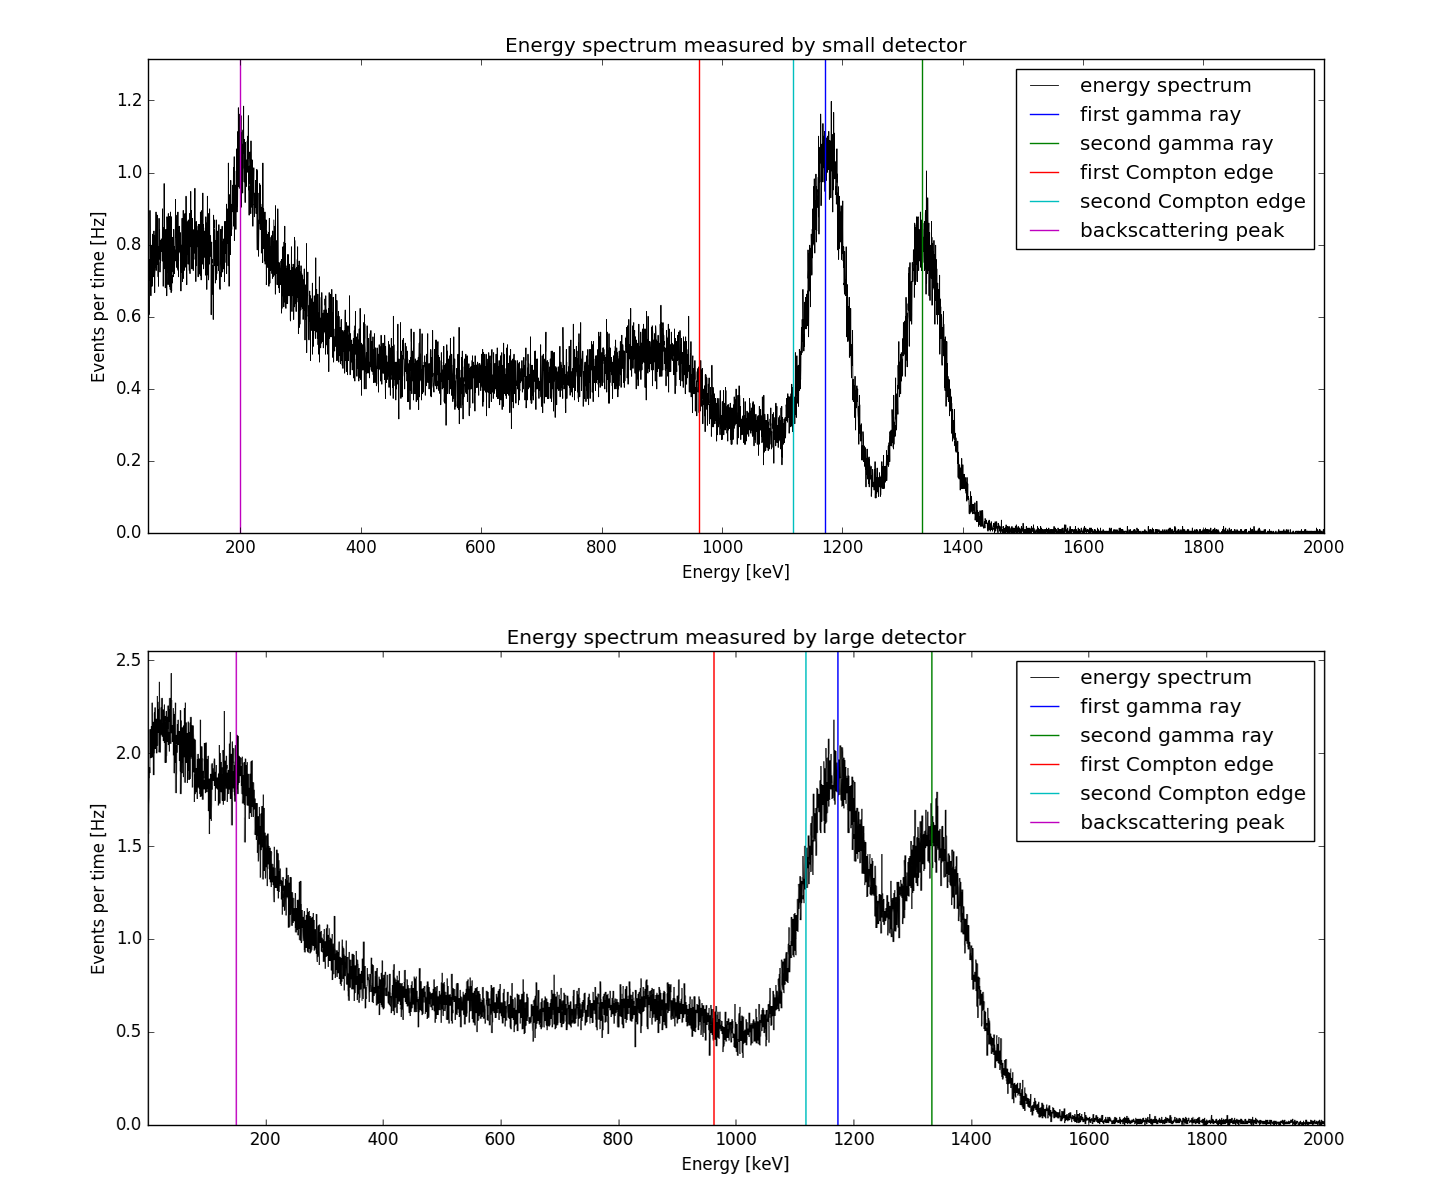
\includegraphics[scale=0.3]{EnergySpectra.png}
\caption[EnergySpectra]{Energy spectra of each detector with tagged $\gamma$-ray absorption lines and typical detection byproducts}
\label{fig:EnergySpectra}
	\end{figure}	
		In addition to the two sharp gamma ray peaks, there is a typical Compton continuum visible on the left. The Compton edge can be obtained as follows [\ref{source:GlennLnoll}]
	\begin{equation}
E_{CE} = E_{\gamma} \cdot \left(1 - \frac{1}{1+2 E_{\gamma}/m_ec^2} \right).
\end{equation}
		This yields a value of $E_{CE,1}$ = 963 keV for the first $\gamma$-ray and $E_{CE,2}$ = 1118 keV for the second $\gamma$-ray. The first Compton edge is clearly visible in the plots while the second one coincides with the finite width of the first $\gamma$-ray line. Thus, it is clear that the Compton continuum does not vanish completely after the first edge.

		There is also an additional peak visible in both plots at around 200 keV in the case of the small detector and 150 keV for the large one. This is a very common effect that can be traced back to backscattering which originates from $\gamma$-rays that have Compton scattered in the material surrounding the detector material before being detected. In the literature, this peak is said to be expected at around 200 keV, which is in very good agreement with the measurement. It also makes sense that this peak is not the same for both detectors, since they are not identical models.


\chapter{Calibration}

\section{Time Calibration}

		Equivalently to the energy calibration in section [\ref{sec:EnergySpectrum}], the MCA transmitted the number of events as a function of the corresponding channel to the computer. In order to convert the channel number to the corresponding physical time delay, a time calibration measurement has been performed. This consisted of connecting the signal of the same detector to the TAC where the copy connected to the stop-channel first passed the delay module. The signal that the TAC induces for various delay settings in the MCA could then be directly observed in the computer. Data was collected and saved for five different delay settings, which can be seen in figure \ref{fig:TimeCal1}. In this case, the number of events in the vertical axis does not contribute any physical meaning.
		\begin{figure}[H]
\centering
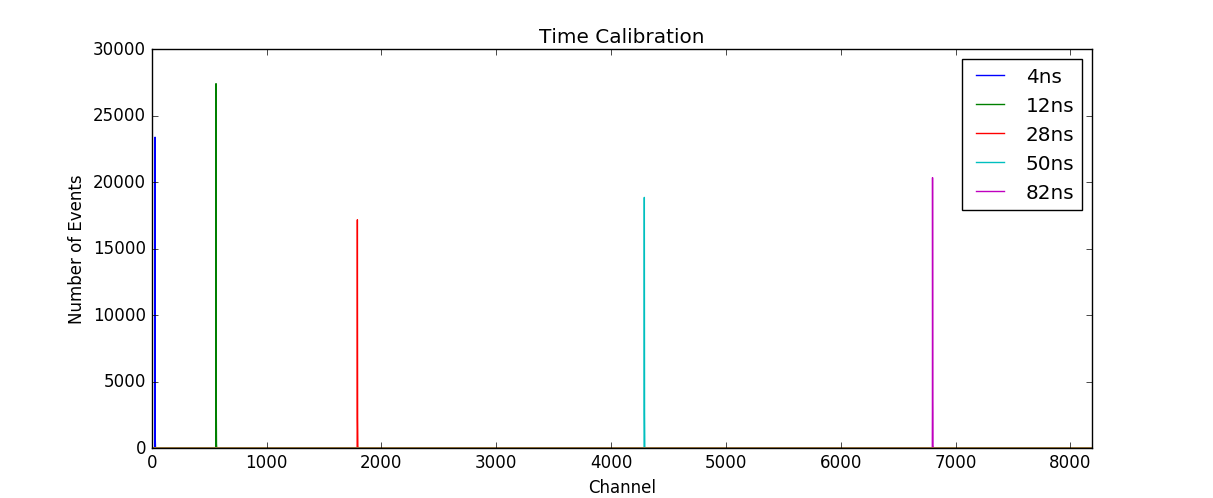
\includegraphics[scale=0.5]{TimeCalibration1.png}
\caption[TimeCalibration1]{Time calibration measurement where each line corresponds to a known delay time}
\label{fig:TimeCal1}
	\end{figure}
	From this, we could deduce which channel corresponds to which magnitude of delay. The channel number and ther corresponding delay time were plotted and a linear fit through the data points could be performed (see figure \ref{fig:TimeCal2}), which yields the following rescaling function:
	\begin{equation}
	time-scale = channel-scale \cdot 0.0111ns + 5.2041ns 
	\end{equation}
	\begin{figure}[H]
\centering
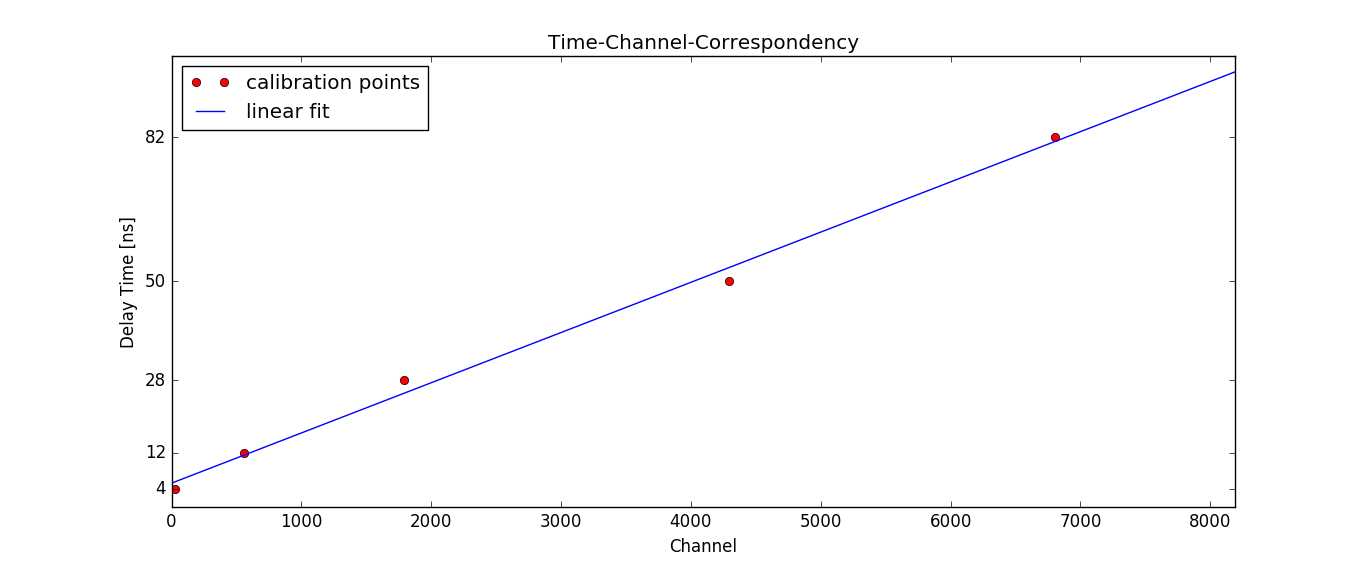
\includegraphics[scale=0.39]{TimeCalibration2.png}
\caption[TimeCalibration2]{Linear fit through the corresponding delay-channel-points}
\label{fig:TimeCal2}
	\end{figure}


\chapter{Appendix}

versprochener unskalierter Energieplot nicht vergessen

\end{document}